\section{Introduction}
With the recent advances of deep learning, integrating the main blocks of automatic speech recognition (ASR) such as acoustic model, pronunciation lexicon and language model into a single framework is highly attractive. Connectionist Temporal Classification (CTC) lends itself on such end-to-end approach by introducing an additional blank symbol and specifically-designed loss function optimizing to generate the correct character sequences from the speech signal directly, without framewise phoneme alignment in advance. With many recent results, end-to-end deep learning has created larger interest in speech community.

Such end-to-end ASR system requires a huge amount of paired speech-transcription data. For most languages in the world, they are lacking of sufficient paired data for training (low-resource). The dominant technique in low-resource setting is to learn language-independent representation of speech signal via multilingual training first, then fine-tune on target language. In such training scheme, inputs from different languages are passed through the shared feed-forward layers, then being passed through language-specific layers to output final character sequences of certrain language.

Various approaches have been proposed based on multilingual training. Langauge-adversarial training approaches introduce language-adversarial classification objective to the shared hidden layers, negating the gradients backproped from the classifier to encourage model to extract more language-independent representations. Hierarchical and multitask approaches introduce different granularity objective through combining both character and phoneme prediction at different levels of the model.

\begin{figure}[htb]

\begin{minipage}[b]{0.48\linewidth}
  \centering
  \centerline{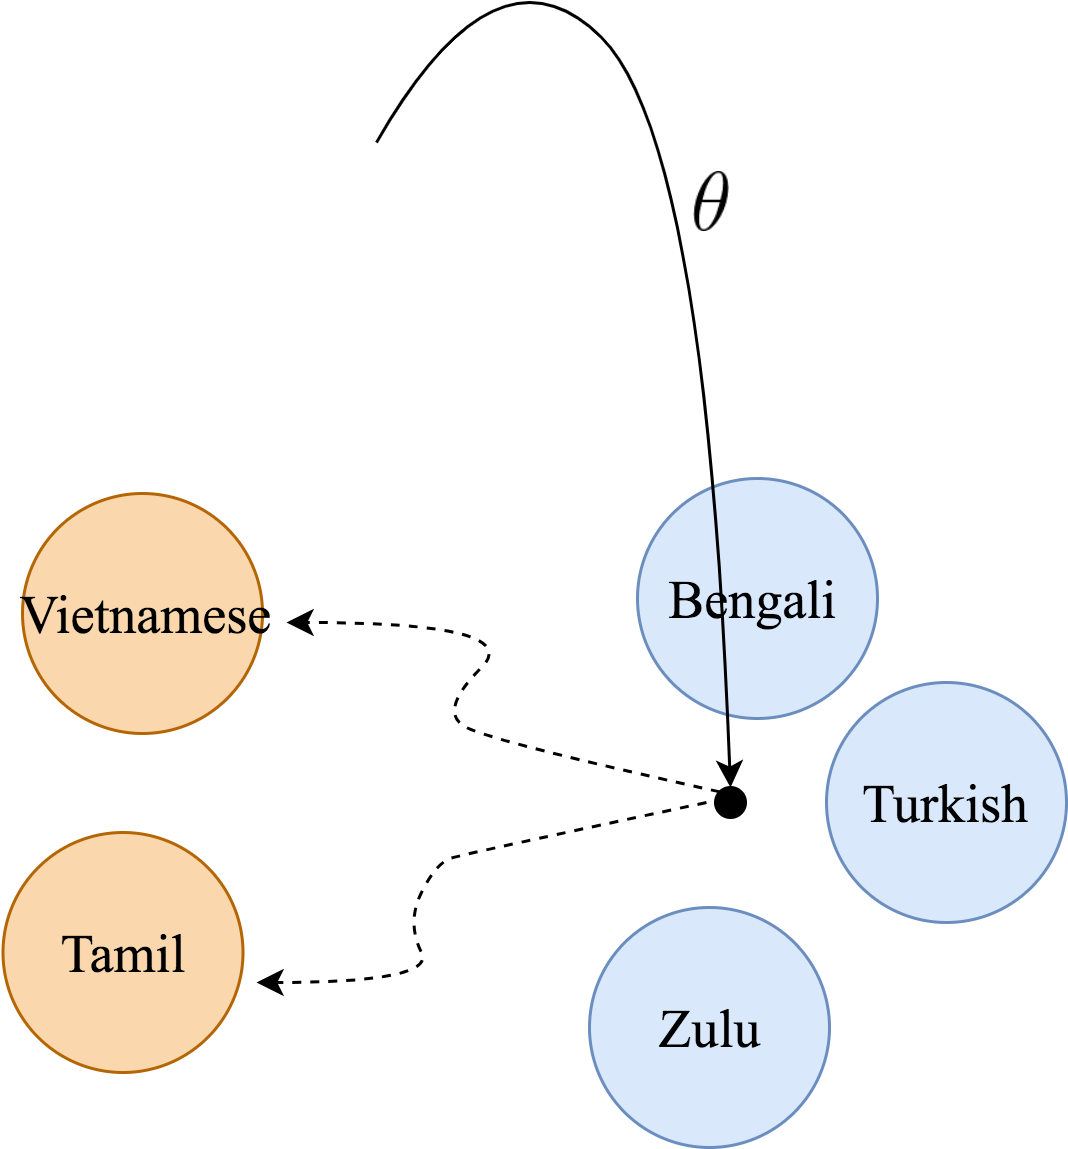
\includegraphics[width=4.0cm]{figs/multi_process.png}}
%  \vspace{1.5cm}
  \centerline{(a) MultiASR}\medskip
\end{minipage}
\hfill
\begin{minipage}[b]{0.48\linewidth}
  \centering
  \centerline{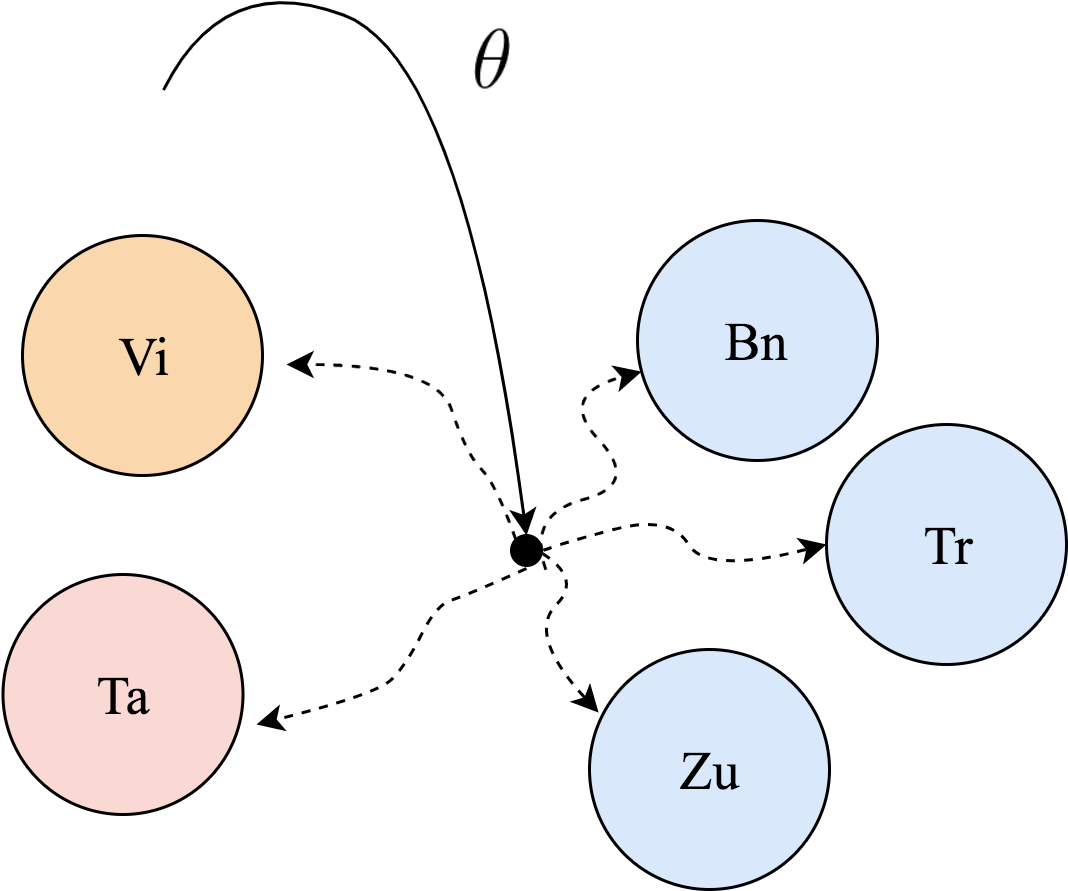
\includegraphics[width=4.0cm]{figs/meta_process.png}}
%  \vspace{1.5cm}
  \centerline{(b) MetaASR}\medskip
\end{minipage}
%
\caption{Illustration: Difference of the learned parameters from MultiASR \& MetaASR. The solid lines represent the learning process of pretraining, either multitask or meta learning. The dashed lines represent the language-specific adaptation.\\ (The figure is modified from \cite{gu2018meta})}
\label{fig:meta-idea}
%
\end{figure}



In this paper, we follow up on the core idea of multilingual training and propose a meta-learning algorithm for low-resource ASR. The goal of meta-learning is to solve the problem of ``fast adaptation on unseen data'', which is aligned with our low-resource setting. There are different aims of meta-learning, such as effective distance metric of samples (metric-based), the policy for updating model parameters (model-based) and good parameter initialization (optimization-based). Meta-learning has already gained many success under few-shot learning setting, and are highly concerned in computer vision community. 

Recently, other than few-shot learning, meta-learning has been successfully used for neural machine translation \cite{gu2018meta}, speaker adaptation \cite{klejch2018learning} and language generation \cite{mi2019meta}. We introduced the recently proposed optimization-based meta-learning approach, model-agnostic meta-learning (MAML) \cite{finn2017model} into the multilingual training scheme by formulating differnet languages as different tasks, and use MAML to find better initialization weights of model to adapt on unseen low-resource language more effectively, and emperically showed that meta-learning can improve the ASR performance on IARPA-BABEL corpus over original multitask training.

\label{sec:intro}

